% Rebuild with pdflatex volume-stacks.tex. Requires standalone and TikZ.
% Each stack is an order ideal in {0,1}^3. The complement exposes the
% three back walls of the hexagonal projection. The four heights are
% listed in the order (0,0), (1,0), (0,1), (1,1).
\documentclass[tikz,border=1mm]{standalone}
\usepackage[T1]{fontenc}
\usepackage{lmodern}
\ifdefined\pdfinfoomitdate\pdfinfoomitdate=1\fi
\ifdefined\pdftrailerid\pdftrailerid{}\fi
\ifdefined\pdfsuppressptexinfo\pdfsuppressptexinfo=15\fi
\pdfinfo{/Title (The twenty stacks in a 2 by 2 by 2 box) /Author (twinheterodox)}

\definecolor{plateInk}{HTML}{223A41}
\definecolor{plateTeal}{HTML}{427E80}
\definecolor{plateOchre}{HTML}{C99143}
\definecolor{wallLine}{HTML}{A7B5B1}
\definecolor{wallFloor}{HTML}{FAF8F1}
\definecolor{wallRight}{HTML}{E6ECE8}
\definecolor{wallLeft}{HTML}{F1F3EF}
\tikzset{
  wall/.style={draw=wallLine,line width=.24pt},
  cube/.style={draw=plateInk,line width=.36pt},
  floor tile/.style={wall,fill=wallFloor},
  far right/.style={wall,fill=wallRight},
  far left/.style={wall,fill=wallLeft},
  cube top/.style={cube,fill=plateOchre!67!white},
  cube right/.style={cube,fill=plateTeal},
  cube left/.style={cube,fill=plateTeal!53!white}
}

% One horizontal lozenge for each column, including zero-height columns.
\newcommand{\TopTile}[3]{%
  \ifnum#3=0\relax\def\tileStyle{floor tile}\else\def\tileStyle{cube top}\fi
  \path[\tileStyle] (#1,#2,#3) -- ({#1+1},#2,#3)
    -- ({#1+1},{#2+1},#3) -- (#1,{#2+1},#3) -- cycle;
}

% Vertical unit faces where the height drops from #4 to #3.
\newcommand{\XStrip}[4]{%
  \ifnum#1=0\relax\def\tileStyle{far right}\else\def\tileStyle{cube right}\fi
  \foreach \level in {0,1}{
    \ifnum\level<#3\relax\else\ifnum\level<#4\relax
      \path[\tileStyle] (#1,#2,\level) -- (#1,{#2+1},\level)
        -- (#1,{#2+1},{\level+1}) -- (#1,#2,{\level+1}) -- cycle;
    \fi\fi
  }%
}
\newcommand{\YStrip}[4]{%
  \ifnum#2=0\relax\def\tileStyle{far left}\else\def\tileStyle{cube left}\fi
  \foreach \level in {0,1}{
    \ifnum\level<#3\relax\else\ifnum\level<#4\relax
      \path[\tileStyle] (#1,#2,\level) -- ({#1+1},#2,\level)
        -- ({#1+1},#2,{\level+1}) -- (#1,#2,{\level+1}) -- cycle;
    \fi\fi
  }%
}
\newcommand{\DrawStack}[4]{%
  \XStrip{0}{0}{#1}{2}\XStrip{1}{0}{#2}{#1}\XStrip{2}{0}{0}{#2}%
  \XStrip{0}{1}{#3}{2}\XStrip{1}{1}{#4}{#3}\XStrip{2}{1}{0}{#4}%
  \YStrip{0}{0}{#1}{2}\YStrip{0}{1}{#3}{#1}\YStrip{0}{2}{0}{#3}%
  \YStrip{1}{0}{#2}{2}\YStrip{1}{1}{#4}{#2}\YStrip{1}{2}{0}{#4}%
  \TopTile{0}{0}{#1}\TopTile{1}{0}{#2}\TopTile{0}{1}{#3}\TopTile{1}{1}{#4}%
  \draw[draw=plateInk!78,line width=.42pt]
     (0,0,2) -- (2,0,2) -- (2,0,0) -- (2,2,0)
       -- (0,2,0) -- (0,2,2) -- cycle;
}

\begin{document}
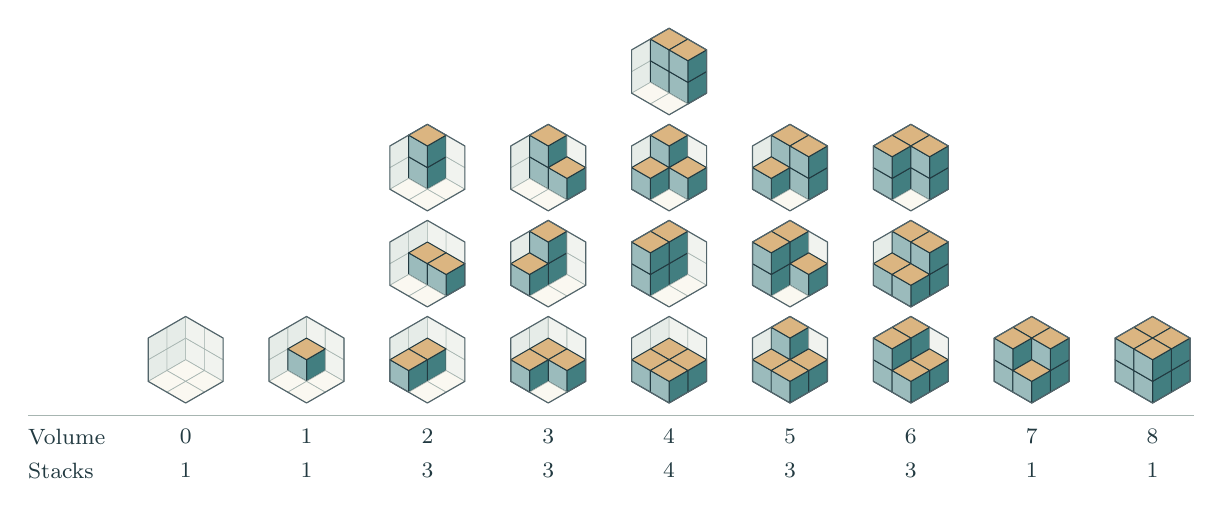
\begin{tikzpicture}[
  x=1mm,y=1mm,line join=round,
  every node/.style={inner sep=0pt,outer sep=0pt,text=plateInk,
                     font=\fontsize{8.4}{9.4}\selectfont}]
  \foreach \v in {0,...,8}{\expandafter\xdef\csname stackCount\v\endcsname{0}}
  \foreach \a in {0,1,2}{\foreach \b in {0,1,2}{
    \foreach \c in {0,1,2}{\foreach \d in {0,1,2}{
      \pgfmathtruncatemacro{\valid}{(\a>=\b)&&(\a>=\c)&&(\b>=\d)&&(\c>=\d)}
      \ifnum\valid=1\relax
        \edef\v{\number\numexpr\a+\b+\c+\d\relax}%
        \edef\rownum{\csname stackCount\v\endcsname}%
        \begin{scope}[shift={({20+15.35*\v},{11+12.2*\rownum})}]
          \begin{scope}[x={(2.38mm,-1.374mm)},y={(-2.38mm,-1.374mm)},
                        z={(0mm,2.748mm)}]
            \DrawStack{\a}{\b}{\c}{\d}
          \end{scope}
        \end{scope}
        \expandafter\xdef\csname stackCount\v\endcsname{\number\numexpr\rownum+1\relax}%
      \fi
    }}%
  }}%
  \draw[draw=wallLine,line width=.36pt] (0,3.95) -- (148,3.95);
  \node[anchor=west] at (0,1.25) {Volume};
  \node[anchor=west] at (0,-3.1) {Stacks};
  \foreach \v/\expected in {0/1,1/1,2/3,3/3,4/4,5/3,6/3,7/1,8/1}{
    \ifnum\csname stackCount\v\endcsname=\expected\relax\else
      \PackageError{volume-stacks}{Incorrect number of stacks of volume \v}{}%
    \fi
    \node at ({20+15.35*\v},1.25) {\v};
    \node at ({20+15.35*\v},-3.1) {\csname stackCount\v\endcsname};
  }
\end{tikzpicture}
\end{document}
